 %!TEX root = ../../report.tex


\subsection{Visualization Improvement Techniques} % (fold)
\label{sub:other_techniques}

This section will present other techniques that can be applied to achieve the performance needed for this work.

\subsubsection{Level of Detail} % (fold)
\label{ssub:level_of_detail}

Level of Detail (LOD) is a technique that is used to improve the performance of the graphic pipeline. This is done by managing the complexity of the objects representation relative to some indicator.
Within this indicators, the most common one is the distance of each object to the viewer. If an object is far from the viewer a decrease on the detail will not be noticed and will save computation time. Other indicators can be the importance that is assigned for each object, relative speed or partial occlusion.

This concept is easy to understand and implement if we look at the example in the Figure~\ref{fig:LOD2}. In this figure there are five cylinders that have different detail according to the distance to the camera. In this case only the number of sides of the cylinder changes.

\begin{figure}[htbp]
	\centering
	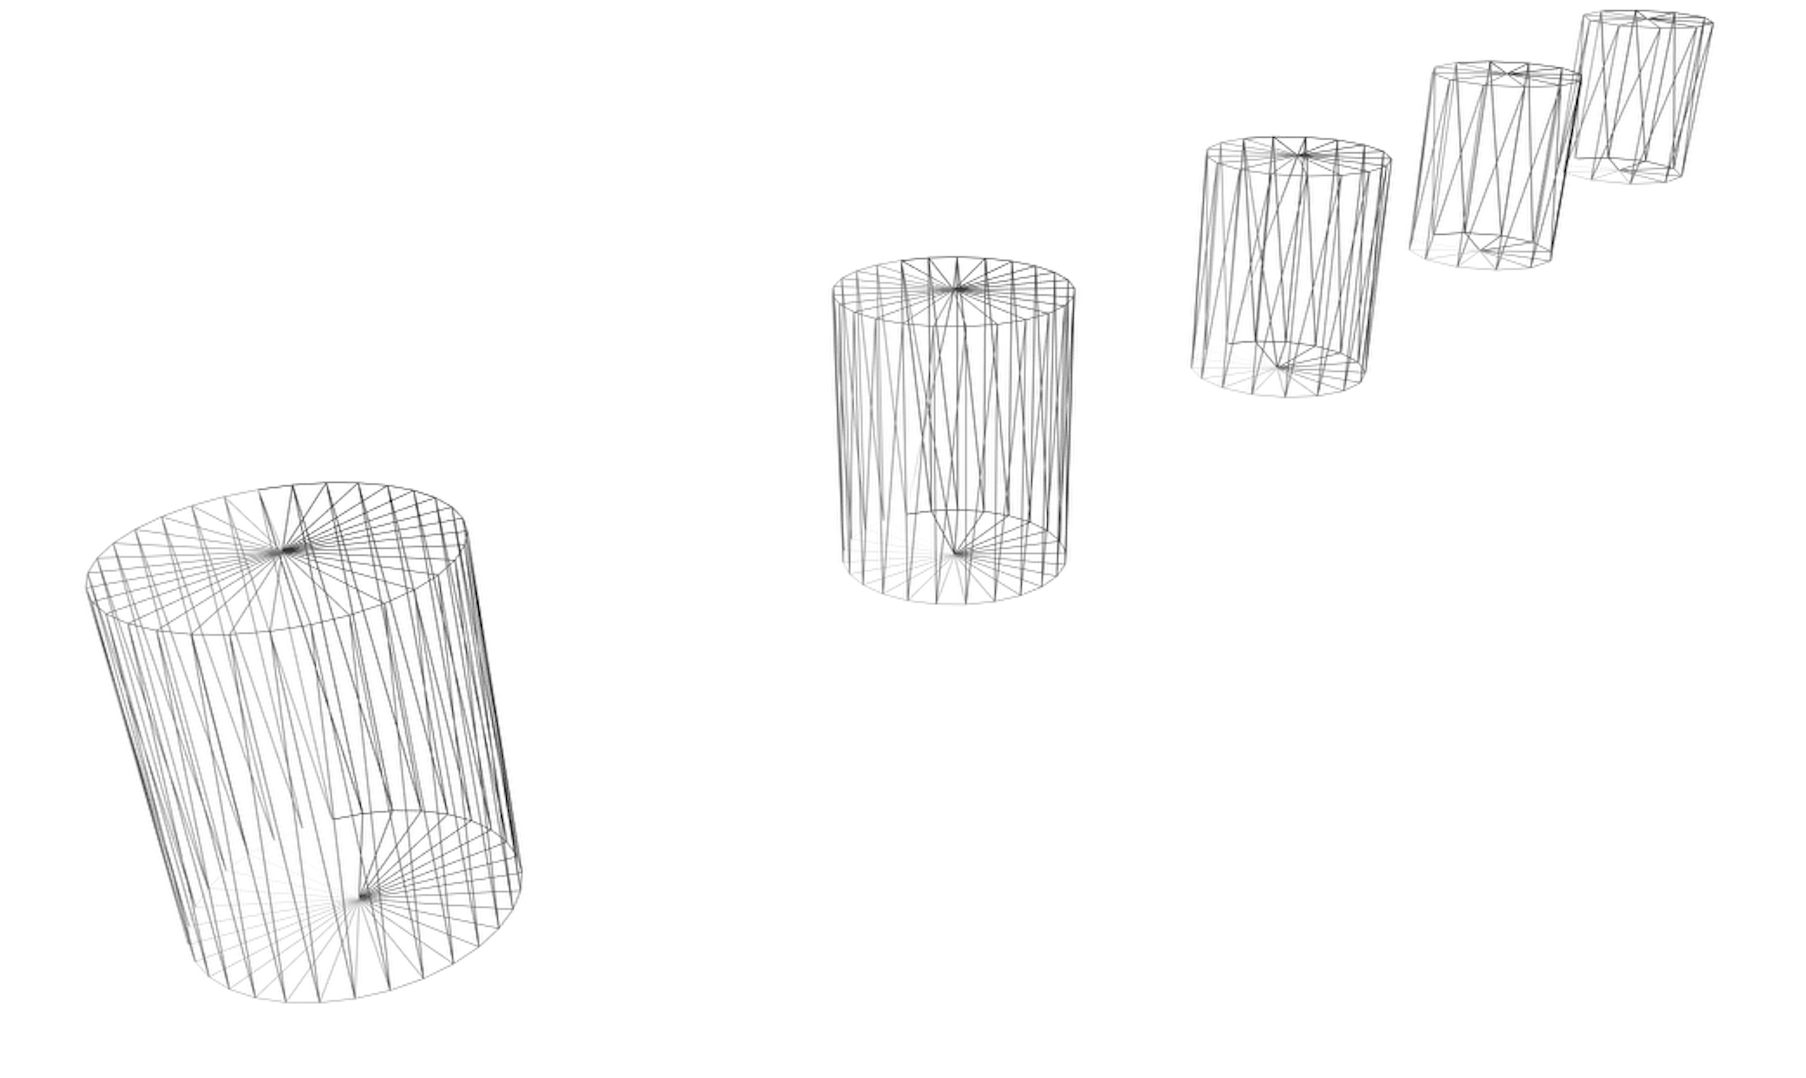
\includegraphics[width=0.95\textwidth]{img/OpenGL/LOD3.png}
	\caption{LOD example}
	\label{fig:LOD2}
\end{figure}
% subsubsection level_of_detail (end)

\subsubsection{Occlusion Culling} % (fold)
\label{ssub:occlusion_culling}

(OC) is another technique that is used to improve performance. It involves determining the faces that are not visible at each point, so that they can be removed from the pipeline.

This technique is usually done automatically by the GPU and applied to occluded faces behind other objects or out of the viewing frustum.

If this concept is applied before the generation of the objects, and prevents the inclusion of large amounts of geometry through the pipeline, we can make a large improvement on performance. Figure~\ref{fig:viewingRange} is a good example. Here only the buildings that are visible from the current point are generated.

% subsubsection occlusion_culling (end)


% subsection other_techniques (end)